\section{Verwendete Methoden Maschinellen Lernens}
\label{sec:lerner}
Zum Verständnis der Ergebnisse müssen zunächst die verwendeten 
Lerner und Methoden erläutert werden, die zur Klassifikation 
und Bewertung der Ergebnisse verwendet werden.

\subsection{Nächste-Nachbarn-Klassifikation}

Der k-Nächste-Nachbarn Klassifikator ist einer der einfachsten Lerner zur 
Klassifikation. Die Klassen werden zugeordnet, in dem die $k$ nächsten Nachbarn 
betrachtet werden. Dabei werden Abstandsmaße verwendet, wie beispielsweise 
euklidische Abstände. Die Wahl des Parameters $k$ hat dabei einen hohen Einfluss 
auf das Ergebniss, da ein zu geringer Wert hohe Sensitivität gegenüber Ausreißern 
hat und ein zu hoher Wert, viele Einträge aus anderen Klassen beinhalten kann. 
In Abbildung \ref{fig:knn} wird die Beeinflussung der Wahl der Anzahl der Nachbarn 
verdeutlicht.

\begin{figure}
  \centering
  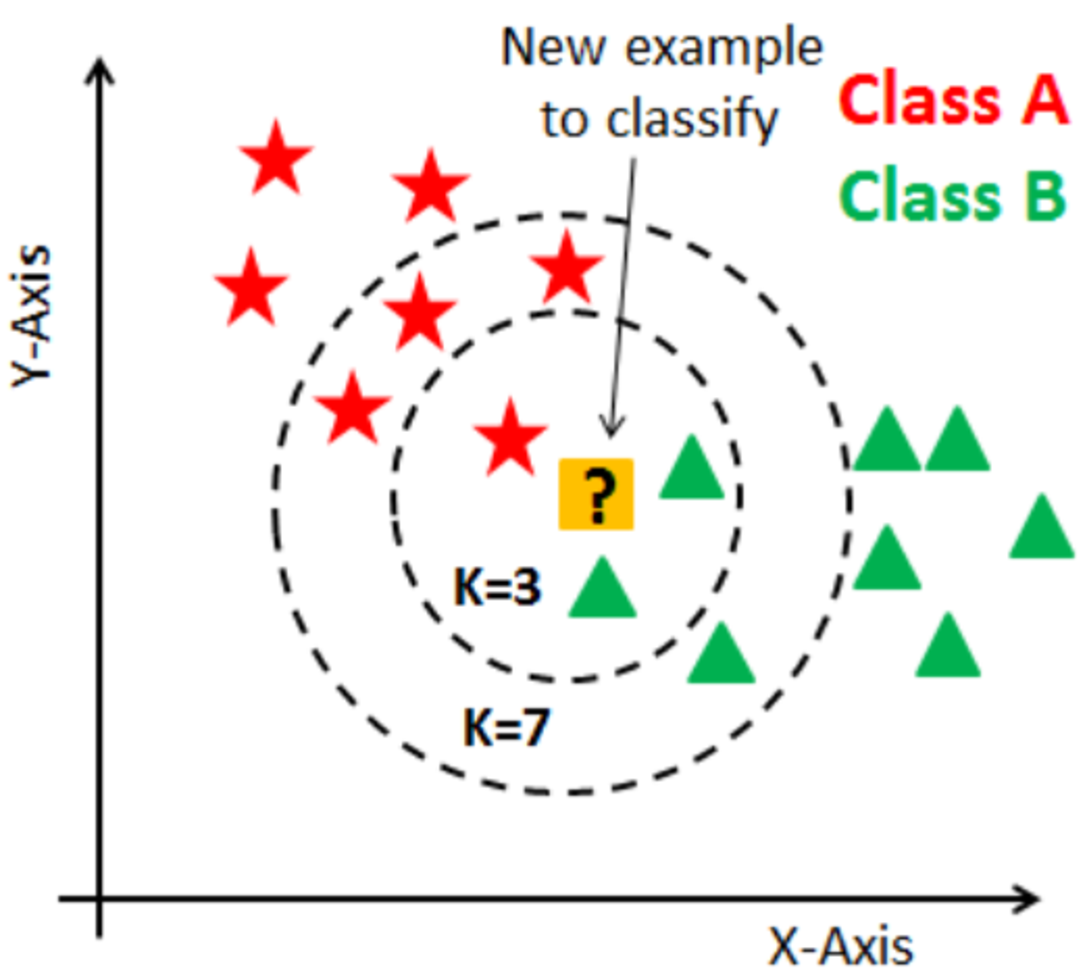
\includegraphics[width=0.5\textwidth]{plots/knn.pdf}
  \caption{Darstellung, wie die Wahl der Anzahl der Nachbarn die Klassifikation des Punktes 
  beeinflussen kann. Bei $k = 3$ wird der Punkt Klasse B zugeordnet. Bei 
  $k = 7$ wird der Punkt Klasse A zugeordnet \cite{kNN}.}
  \label{fig:knn}
\end{figure}

Ein
wichtiger Punkt des kNN-Lerners ist, dass er ein sogenannter \textit{lazy learner} 
ist. Das bedeutet, beim Trainieren werden die Daten lediglich abgespeichert und 
die Klassifikation findet nicht zeitgleich oder im Anschluss an das Training 
statt, sondern erst, wenn die Klassifikation angefordert wird. 


\subsection{Random Forest Klassifikationsverfahren}
Der \texttt{RandomForestClassifier} basiert auf binären Entscheidungsbäumen.
Bei einem Entscheidungsbaum wird an jedem Knoten ein Schnitt in einer Variable durchgeführt und die daraus entstandenen Teilmengen 
werden in den beiden Ästen des Knotens wiederum durch Schnitte unterteilt, bis entweder eine bestimmte Tiefe
des Baumes erreicht ist oder die Blätter nur Ereignisse einer Klasse enthalten. Um die Effekte des Übertrainierens zu minimieren, wird über ein Ensemble unterschiedlicher
Entscheidungsbäume gemittelt.
Die Bäume werden dabei jeweils auf unterschiedlichen Teilmengen des Trainingsdatensatzes trainiert.
Die Attribute des Baumes an denen der beste Schnitt gesucht wird, werden zufällig ausgesucht.

\subsection{Naive-Bayes-Klassifikator}

\subsection{Kreuzvalidierung}

\subsection{Der Jaccard-Index}

\subsection{ROC-Kurven}